\documentclass[conference]{IEEEtran}
\usepackage{cite}
\usepackage{amsmath,amssymb,amsfonts}
\usepackage{algorithm}
\usepackage{algorithmic}
\usepackage{graphicx}
\usepackage{textcomp}
\usepackage{xcolor}
\usepackage{multicol}
\usepackage{float}
\usepackage[spanish]{babel}
\def\BibTeX{{\rm B\kern-.05em{\sc i\kern-.025em b}\kern-.08em
    T\kern-.1667em\lower.7ex\hbox{E}\kern-.125emX}}
\begin{document}

\title{Esteganografía}
\author{\IEEEauthorblockN{Joaquín Pérez Araya}
\IEEEauthorblockA{\textit{Departamento de Ciencias de la Computación} \\
\textit{Universidad de Chile}\\
Santiago, Chile \\
joaquin.perez.a@ug.uchile.cl}}


\maketitle

\begin{abstract}

\end{abstract}

\section*{Introducción} % ***Así la cosa no me molesta con los numeritos***
    A lo largo de la historia de la humanidad ha existido la necesidad de envíar información ocultos, ya sea para transmitir información sensible, como  Ejemplos...
    Uno de los modos es a través de la Esteganografía, que viene de ...
    En este documento se mencionará una implementación de Esteganografía sobre imagenes ... que consiste en ... la
    ... ejemplos de Esteganografía en imagenes (usar \cite{DIS})
    más específicamente un método bastante simple que consiste en...
    (tablita, algoritmo bonito, blablabla)

    Dentro del texto actúal     
    
\section*{Diseño e Implementación}
	Para la implementación del programa se utilizó Python 3.6 con las librerías \texttt{numpy} y     
	\texttt{scimage} y \texttt{argparse}. El código está dividido en 4 partes: Utilidades, Entrada/Salida, Codificación y Decodificación.
\subsection*{Entrada y Salida}
    Para el uso externo del programa por medio de comandos se utilizó la librería \texttt{argparse} que viene por defecto en Python. Leer los comandos dados y traducirlos a llamados directos a las funciones de codificación o decodificación.
    	
	\subsection*{Utilidades}
	El módulo de utilidades (\texttt{util.py}) están las funciones auxiliares que utilizan la codificación y decodificación entre las de las cuales se destacan:
	\begin{itemize}
	    \item \texttt{image\_read}\footnotemark, \texttt{image\_write} y \texttt{text\_read}: Son las funciones para leer los archivos externos que se van a utilizar para el proceso de codificación y decodificación.
         
	    \footnotetext{La función que está implementada en el código es la que está en \texttt{pai\_io.py} dentro del repositorio del curso.}
	    	    
        \item \texttt{text\_to\_ascii} y \texttt{ascii\_to\_text}: La primera se utiliza para codificar el mensaje mientras que la segunda para decodificar. Se usan para transformar una cadena de texto a una lista de números donde cada caracter es un número de la lista y viceversa.
        
        \item \texttt{to\_binary} y \texttt{to\_int}: Se utilizan para codificar y decodificar, ya que reduce el problema de inserción de bits a modificar las cadenas de texto en binario de los valores del canal de imagen.
        
        \item \texttt{join\_binaries}: Se usa modificar la cadena de texto binaria para codificar un caracter en éste.
        
        \item \texttt{last\_value}: Se utiliza para obtener los bits menos significativos de un número, para obtener el caracter que está codificado es éste.
	\end{itemize}
	
	\subsection*{Codificación}
        La codificación consta de una única función que dada la una dirección de imagen, una dirección texto y un número de bits realice todo el proceso de abrir la imagen, obtener el primer canal de información para modificarlo con la finaldiad de agregarle la información que corresponde al texto.
        Dado el primer canal de la imagen dada, se codifica en los cuatros bits menos significativos el número de bits que se van a usar en los siguientes pixieles para facilitar la acción de decodificación.
        Posteriormente, se convierte el texto a codificar a una lista de números donde letra se le asigna un número que corresponde al valor en \texttt{ASCII} del caracter.
    
        Dado a que cada símbolo en \texttt{ASCII} es un número de 8 bits, en cada píxel se puede elegir la cantidad de bits a codificar, éste método permite codificar $\lfloor(p-1)(bits / 8)\rfloor - 1$ caracteres como máximo dentro de una imagen con $p$ píxeles en total, ya que en el primer pixel de la imagen siempre se va a utilizar para guardar la cantidad de bits utilizado en los 4 bits menos significativos de éste, tambien se necesita codificar un caracter adicional para indicar que no se debe seguir decodificando.
        
        
\section*{Experimentación}
    Inicialmente para el testeo del funcionamiento inicial de la implementación se utilizó una imagen en negro de \texttt{10x10} pixeles con la finalidad de verificar vía simple inspección la codificación/decodificación. \\
    
\begin{figure}[H]
\begin{multicols}{4}
    \centering
    
\includegraphics[width=0.9\linewidth]{image/black1.png} \par
    
\includegraphics[width=0.9\linewidth]{image/black2.png} \par
    
\includegraphics[width=0.9\linewidth]{image/black3.png} \par
    
\includegraphics[width=0.9\linewidth]{image/black4.png} \par
    \end{multicols}
    \begin{multicols}{4}
    \centering
    
\includegraphics[width=0.9\linewidth]{image/black5.png} \par
    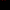
\includegraphics[width=0.9\linewidth]{image/black6.png} \par
    
\includegraphics[width=0.9\linewidth]{image/black7.png} \par
    
\includegraphics[width=0.9\linewidth]{image/black8.png} \par 
\end{multicols}
\caption{El texto \texttt{Hola}, codificado usando 1 a 8 bits.}
\end{figure}



    


\section*{Conclusión}
	Muy bien me gusto, pongame un 7.0 tkm


\begin{thebibliography}{99}
\bibitem{DIS} Cheddad, A., Condell, J., Curran, K., \& Mc Kevitt, P. (2010). Digital image 
steganography: Survey and analysis of current methods. Signal Processing, 90(3), 727–752. 


\end{thebibliography}


\end{document}
